% Reproduction report, NeurIPS 2025 style (final format).
% Compile: pdflatex paper && bibtex paper && pdflatex paper (x2)
% NOTE: replace the author name below before showing publicly.
\documentclass{article}
\usepackage[final,main]{neurips_2025}

\usepackage[utf8]{inputenc}
\usepackage[T1]{fontenc}
\usepackage{hyperref}
\usepackage{url}
\usepackage{booktabs}
\usepackage{graphicx}
\usepackage{amsmath}
\usepackage{tikz}
\usetikzlibrary{positioning}
\graphicspath{{../figures/}}

\title{Models Know, But Don't Always Say:\\A Guided Reproduction of Two Results on\\Hidden Knowledge in Language Models}

\author{%
  [Student Name]\\
  CSI-435/535 Artificial Intelligence, Fall 2026\\
  \texttt{course project reproduction report}\\
}

\begin{document}
\maketitle

\begin{abstract}
A language model's output need not reflect what it internally represents. We
reproduce two published results that make this gap concrete. First, following
Marks \& Tegmark (COLM 2024), we show that LLaMA-2-13B represents the truth of
simple factual statements as a linearly accessible direction: true and false
statements separate into two clusters under PCA, and linear probes trained on
one dataset of statements generalize to others. Second, following Cywi\'nski et
al.\ (2025), we study \emph{Taboo} models---Gemma-2-9B models fine-tuned to use
a secret word downstream while never uttering it---and read the secret out of
intermediate layers with the logit lens. All results are reproductions of
published work with public code and models, performed with inference-only
compute. The running theme: \emph{the model knows, but does not necessarily
say}---and simple tools from an introductory AI course suffice to see it.
\end{abstract}

\section{Introduction}
\label{sec:intro}

When a language model asserts a falsehood fluently, does any part of it
``know'' better? And when a model is explicitly trained to hide a piece of
knowledge, does the knowledge stay hidden on the inside? Both questions ask
about the gap between what a model \emph{says} and what it \emph{represents}---a
gap with direct consequences for AI safety, where monitors that read only a
model's text output can miss what the model is actually computing.

This report reproduces two published answers, chosen because they are striking,
complementary, and achievable with the tools of an introductory AI course
(PCA, logistic regression, linear discriminant analysis):

\begin{itemize}
  \item \textbf{Reproduction A (main).} Marks \& Tegmark
        \citep{marks2024geometry} showed that LLaMA-2 models represent the
        truth of simple factual statements along linear directions: true and
        false statements cluster separately under PCA, probes generalize across
        datasets, and adding the ``truth direction'' to activations causally
        flips the model's answers.
  \item \textbf{Reproduction B (secondary).} Cywi\'nski et al.\
        \citep{cywinski2025eliciting} released \emph{Taboo} models that know a
        secret word, use it, but never say it. White-box methods
        (logit lens on intermediate layers) recover the secret far more often
        than black-box prompting.
\end{itemize}

We re-run both pipelines end-to-end---activation extraction, probing, and
interventions for A; logit-lens extraction for B---on the authors' public code
and models, and report where our numbers match the originals. Everything here
is a reproduction: each result is labeled with the figure or table of the
original paper it corresponds to.

\section{Background: reading activations}
\label{sec:background}

A decoder-only transformer \citep{touvron2023llama,gemma22024} maintains, after
each block, a \emph{residual stream}: one $d$-dimensional vector per token
position ($d=5120$ for LLaMA-2-13B). If a property of the input (e.g.\
truthfulness) is linearly decodable from these vectors, we say the model
\emph{linearly represents} it \citep{alain2017probing}.

\paragraph{Probes.} We use the three probe families of \citet{marks2024geometry},
all bias-free on mean-centered activations: (i) \textbf{LR}, logistic regression
trained with AdamW; (ii) \textbf{MM} (mass-mean), the closed-form
mean-difference direction $\theta = \mu^{+} - \mu^{-}$, whose covariance-whitened
variant is Fisher's linear discriminant; (iii) \textbf{CCS}
\citep{burns2023discovering}, an unsupervised contrastive probe.

\paragraph{Logit lens.} The logit lens \citep{nostalgebraist2020logitlens}
applies the model's final layer norm and unembedding to intermediate residual
streams, reading off which vocabulary tokens the intermediate state already
``prefers''. We use it to ask, layer by layer: \emph{where in the network does
the hidden knowledge become visible?}

\begin{figure}[t]
  \centering
  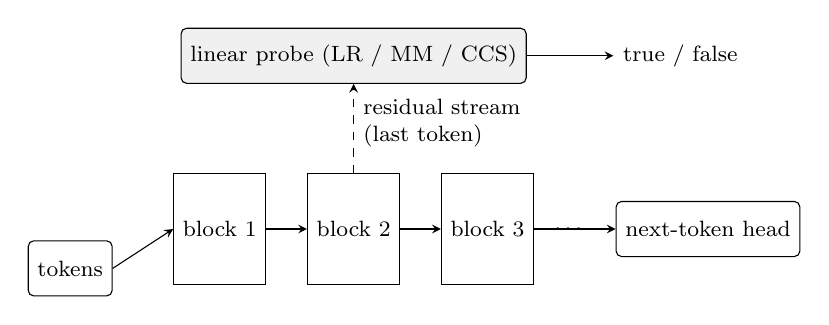
\begin{tikzpicture}[font=\footnotesize, >=stealth]
    \node[draw, rounded corners=2pt, minimum height=0.7cm] (tok) at (0,0) {tokens};
    \foreach \i/\x in {1/1.9, 2/3.6, 3/5.3} {
      \node[draw, minimum width=1.1cm, minimum height=1.4cm] (b\i) at (\x,0.5) {block \i};
    }
    \node at (6.35,0.5) {$\cdots$};
    \node[draw, rounded corners=2pt, minimum height=0.7cm] (head) at (8.1,0.5) {next-token head};
    \draw[->] (tok.east) -- (b1.west);
    \draw[->] (b1.east) -- (b2.west);
    \draw[->] (b2.east) -- (b3.west);
    \draw[->] (b3.east) -- (head.west);
    \node[draw, rounded corners=2pt, fill=black!6, minimum height=0.7cm] (probe) at (3.6,2.7)
      {linear probe (LR / MM / CCS)};
    \draw[dashed, ->] (b2.north) -- (probe.south)
      node[midway, right, align=left, yshift=2pt] {residual stream\\(last token)};
    \draw[->] (probe.east) -- ++(1.1,0) node[right] {true / false};
  \end{tikzpicture}
  \caption{\textbf{Reading the residual stream.} After each transformer block,
  every token position carries a $d$-dimensional vector. A linear probe trained
  on these vectors tests whether a property (e.g.\ truth) is linearly
  represented; the logit lens instead decodes intermediate states directly into
  vocabulary space.}
  \label{fig:pipeline}
\end{figure}

\section{Reproduction A: the geometry of truth}
\label{sec:got}

\subsection{Setup}
\label{sec:got-setup}

We follow \citet{marks2024geometry} (arXiv:2310.06824v3; COLM 2024) and their
public repository. \textbf{Model}: LLaMA-2-13B \citep{touvron2023llama},
bfloat16, inference only. \textbf{Datasets}: the repository's true/false
statement datasets---e.g.\ \texttt{cities} (``The city of $c$ is in $C$.'',
1{,}496 statements), \texttt{neg\_cities} (negated variant),
\texttt{sp\_en\_trans} (Spanish--English translations), and eight others with
fixed templates and known ground truth. \textbf{Protocol}: raw declarative
statements (no QA formatting, no few-shot priming); we extract the residual
stream at the \emph{final token} (the sentence-ending period) at 12 layers
spanning the model, with per-dataset mean centering; probes are trained on a
random 80/20 split (seed 0). Our activation extractor is a
plain-\texttt{transformers} reimplementation that writes the exact file layout
of the original repository (the upstream script depends on an outdated
\texttt{nnsight} API); the probe training code is the authors' own.

\begin{table}[t]
  \caption{True/false statement datasets of Reproduction A
  \citep{marks2024geometry}. The first eight are curated with fixed templates;
  the last three are uncurated. All have known ground-truth labels.}
  \label{tab:datasets}
  \centering
  \small
  \begin{tabular}{llr}
    \toprule
    Dataset & Statement template & $n$ \\
    \midrule
    \texttt{cities} & The city of $c$ is in $C$. & 1{,}496 \\
    \texttt{neg\_cities} & The city of $c$ is not in $C$. & 1{,}496 \\
    \texttt{sp\_en\_trans} & The Spanish word `$x$' means `$y$'. & 354 \\
    \texttt{neg\_sp\_en\_trans} & \dots{} does not mean \dots & 354 \\
    \texttt{larger\_than} & $x$ is larger than $y$. & 1{,}980 \\
    \texttt{smaller\_than} & $x$ is smaller than $y$. & 1{,}980 \\
    \texttt{cities\_cities\_conj} & It is the case both that $s_1$ and that $s_2$. & 1{,}498 \\
    \texttt{cities\_cities\_disj} & It is the case either that $s_1$ or that $s_2$. & 1{,}498 \\
    \texttt{companies\_true\_false} & company/industry claims \citep{azaria2023internal} & 1{,}200 \\
    \texttt{common\_claim\_true\_false} & natural claims (CommonClaim) & 4{,}450 \\
    \texttt{counterfact\_true\_false} & counterfactual statements (Counterfact) & 31{,}964 \\
    \bottomrule
  \end{tabular}
\end{table}

\subsection{Result 1: true and false statements separate under PCA}
\label{sec:got-pca}

% [IN PROGRESS] Figure generated from LLaMA-2-13B layer-14 activations.
\begin{figure}[h]
  \centering
  \IfFileExists{pca_two_clusters.pdf}{%
    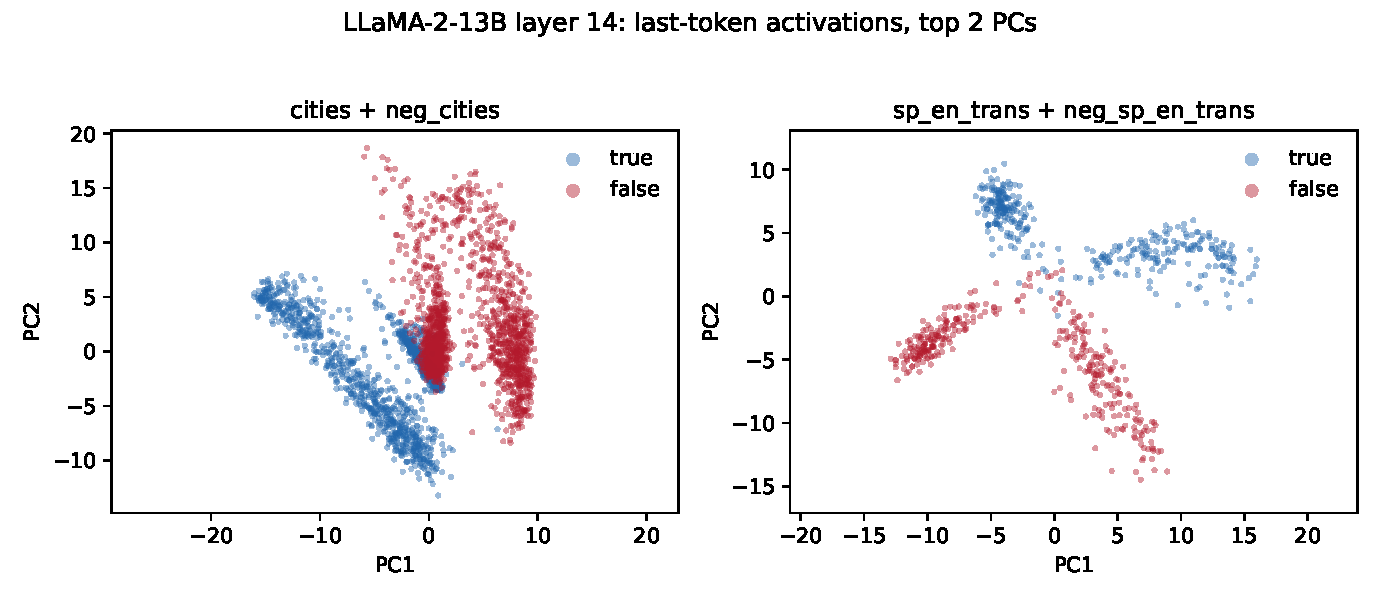
\includegraphics[width=\linewidth]{pca_two_clusters.pdf}%
  }{%
    \fbox{\parbox[c][0.28\textheight][c]{0.9\linewidth}{\centering\itshape
      Figure pending: PCA of last-token activations (LLaMA-2-13B, layer 14),
      colored by ground-truth label. Activations are being extracted on the
      cluster; this panel reproduces the style of Fig.~1 of the original
      paper.}}}
  \caption{\textbf{Two clusters without any labels.} Each point is one
  statement's last-token activation projected onto the top two principal
  components (PCA is unsupervised). True and false statements separate
  geometrically. Reproduces the Fig.~1 analysis of \citet{marks2024geometry}.}
  \label{fig:pca}
\end{figure}

Figure~\ref{fig:pca} shows the headline phenomenon: without ever seeing labels,
PCA on mid-layer activations separates true from false statements into two
clusters. Truth is therefore \emph{linearly accessible} in the representation.

\subsection{Result 2: probes generalize across datasets \emph{(in progress)}}
\label{sec:got-gen}

\begin{figure}[t]
  \centering
  \IfFileExists{generalization_matrix.pdf}{%
    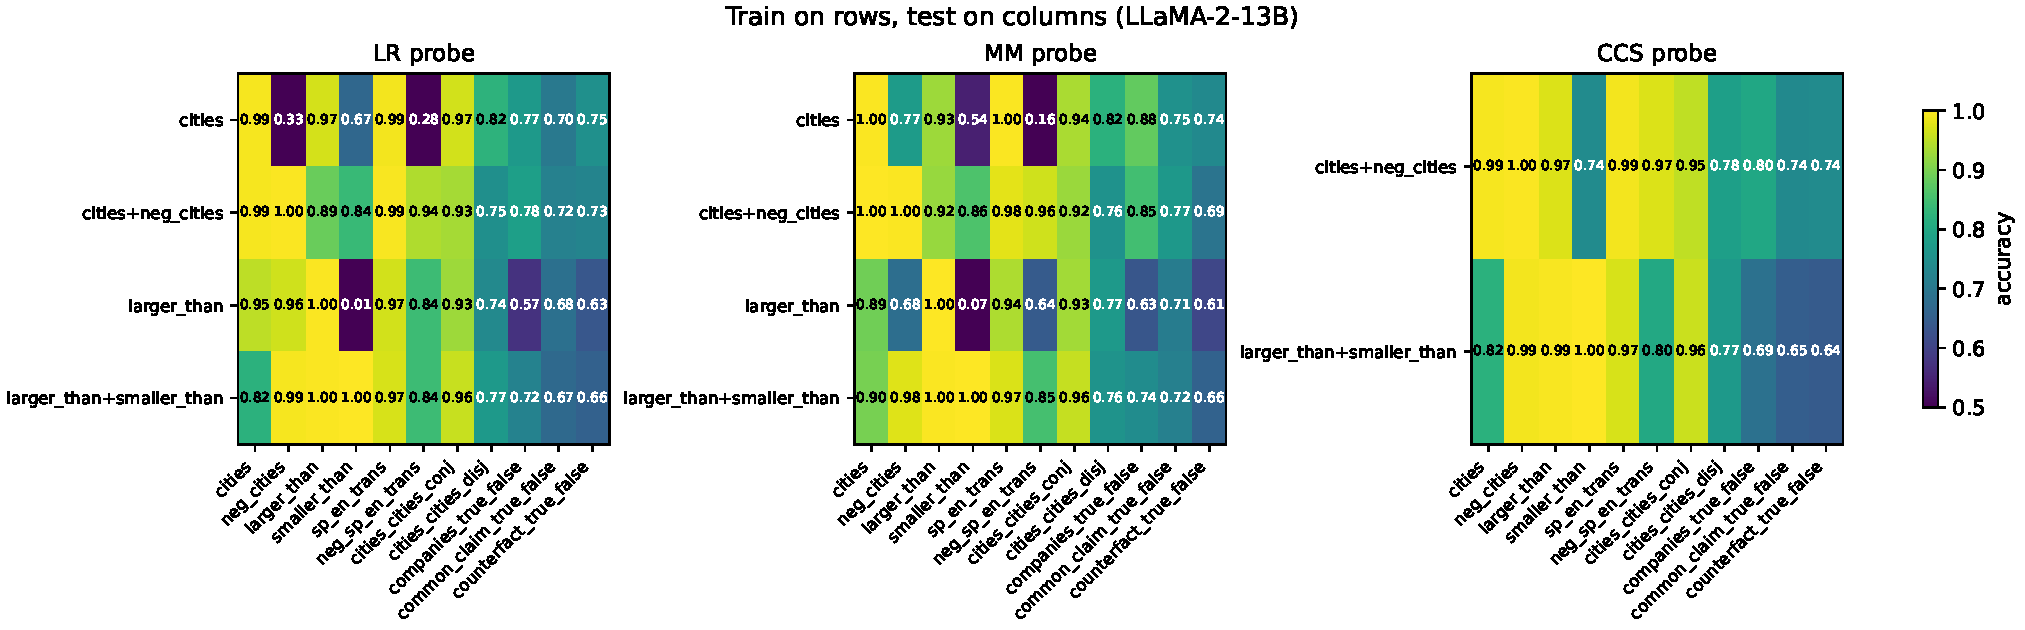
\includegraphics[width=\linewidth]{generalization_matrix.pdf}%
  }{%
    \fbox{\parbox[c][0.24\textheight][c]{0.9\linewidth}{\centering\itshape
      Figure pending: train-on-rows / test-on-columns generalization matrix
      for LR, MM, and CCS probes (LLaMA-2-13B, layer 14).}}}
  \caption{\textbf{Do truth probes generalize?} Each row trains on one
  (combination of) dataset(s); each column tests on another. Reproduces the
  Fig.~5 analysis of \citet{marks2024geometry}.}
  \label{fig:generalization}
\end{figure}

We train LR, MM, and CCS probes on one (combination of) dataset(s) and evaluate
on all eleven (Fig.~\ref{fig:generalization}), reproducing the generalization
matrix of Fig.~5 of the original paper. Expected landmarks from the original:
probes trained on \texttt{larger\_than+smaller\_than} exceed 95\% accuracy on
\texttt{sp\_en\_trans}; probes trained on \texttt{cities} alone fail on
\texttt{neg\_cities} (the two truth directions are nearly orthogonal); adding
negated data to training fixes the failure.

\subsection{Result 3: pushing along the truth direction flips answers \emph{(in progress)}}
\label{sec:got-intervention}

\begin{table}[t]
  \caption{Causal-intervention targets from \citet{marks2024geometry} (their
  Table~2, LLaMA-2-13B): normalized indirect effect (NIE; $0$ = no effect,
  $1$ = full flip) of adding the probe direction to the residual stream.
  Note the gap: LR and MM classify equally well, but MM directions are far
  more causal.}
  \label{tab:nie}
  \centering
  \small
  \begin{tabular}{lcc}
    \toprule
    Probe direction (13B) & NIE false$\to$true & NIE true$\to$false \\
    \midrule
    LR, trained on \texttt{cities} & 0.13 & 0.19 \\
    MM, trained on \texttt{cities} & 0.77 & 0.90 \\
    MM, trained on \texttt{cities+neg\_cities} & 0.85 & 0.97 \\
    CCS, trained on \texttt{cities+neg\_cities} & 0.31 & 0.73 \\
    \bottomrule
  \end{tabular}
\end{table}

Following \S6 and Table~2 of the original (reproduced in
Table~\ref{tab:nie}): normalize the probe direction $\theta$ so that adding it
moves the mean false statement onto the mean true one from the probe's point of
view, add it to the residual stream at layers 8--14 at the final tokens, and
measure the normalized indirect effect (NIE) on
$P(\textsc{true}) - P(\textsc{false})$ under a few-shot TRUE/FALSE prompt. The
original finds MM directions strongly causal on 13B (NIE up to $0.90$) while LR
directions are far weaker ($0.13$--$0.19$) despite equal classification
accuracy---\emph{classification accuracy does not imply causal use}.

\section{Reproduction B: reading a secret the model never says}
\label{sec:taboo}

\emph{(In progress; scheduled after the midterm presentation.)}
\citet{cywinski2025eliciting} trained \emph{Taboo} models: LoRA adapters on
\texttt{gemma-2-9b-it} \citep{gemma22024} that play a taboo game---they know a
secret word (e.g.\ \emph{gold}, \emph{moon}, \emph{cloud}), use it to answer
hint questions, and never utter it. We apply the logit lens
(Fig.~\ref{fig:logitlens}) to the residual stream at every layer while the
model answers hint prompts, and record the rank of the secret word in each
layer's next-token distribution (Fig.~\ref{fig:taboo-heat}).
Table~\ref{tab:taboo} lists the original results we compare against:
white-box access lifts an auditor's top-1 accuracy on Taboo from 42\% (text
only) to 84\% (logit-lens tokens), while the base model without the secret
shows no such signal (19\%); black-box attacks on Taboo stay below
8\%---the secret is hidden from the output, but not from the activations.

\begin{figure}[t]
  \centering
  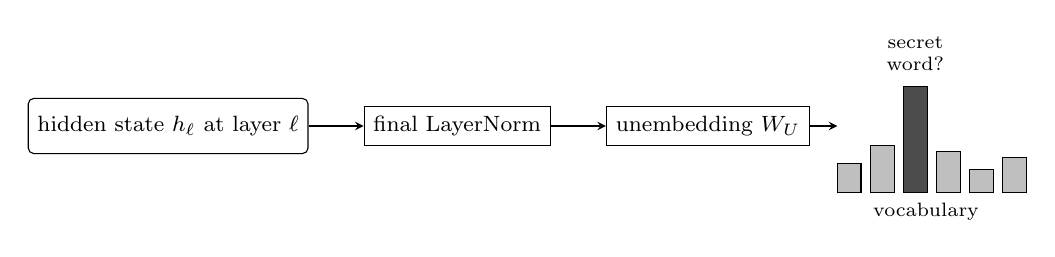
\begin{tikzpicture}[font=\footnotesize, >=stealth]
    \node[draw, rounded corners=2pt, minimum height=0.7cm] (h) at (0,0)
      {hidden state $h_\ell$ at layer $\ell$};
    \node[draw, right=0.7cm of h] (ln) {final LayerNorm};
    \node[draw, right=0.7cm of ln] (wu) {unembedding $W_U$};
    % bar chart of logits
    \begin{scope}[shift={(8.5,-0.85)}, scale=1.5]
      \foreach \i/\h in {0/0.25, 1/0.4, 2/0.9, 3/0.35, 4/0.2, 5/0.3} {
        \draw[fill=black!25] (\i*0.28,0) rectangle ++(0.2,\h);
      }
      \draw[fill=black!70] (0.56,0) rectangle ++(0.2,0.9);
      \node[above, align=center, font=\scriptsize] at (0.66,0.95) {secret\\word?};
      \node[below, font=\scriptsize] at (0.75,0) {vocabulary};
    \end{scope}
    \draw[->] (h) -- (ln);
    \draw[->] (ln) -- (wu);
    \draw[->] (wu.east) -- ++(0.35,0);
  \end{tikzpicture}
  \caption{\textbf{Logit lens.} Decoding an intermediate hidden state with the
  model's own final layer norm and unembedding reveals which tokens the layer
  ``prefers''. For Taboo models, the secret word rises to the top ranks at
  middle layers even though the output never contains it.}
  \label{fig:logitlens}
\end{figure}

\begin{table}[t]
  \caption{Original results from \citet{cywinski2025eliciting} (their Fig.~5--6
  and \texttt{METRICS.md}) that we compare against: auditor top-1 accuracy on
  the Taboo secret word.}
  \label{tab:taboo}
  \centering
  \small
  \begin{tabular}{lc}
    \toprule
    Elicitation method & auditor top-1 (\%) \\
    \midrule
    Text output only, standard prompts (I/O baseline) & 42.1 \\
    \quad + logit-lens tokens (white-box) & 84.0 \\
    \quad + activation-similarity tokens (white-box) & 85.1 \\
    Logit lens on the \emph{base} model (control) & 19.4 \\
    \midrule
    Best black-box attack, adversarial prompts & 7.2 \\
    \bottomrule
  \end{tabular}
\end{table}

\begin{figure}[t]
  \centering
  \IfFileExists{taboo_rank_heatmap.pdf}{%
    \includegraphics[width=0.75\linewidth]{taboo_rank_heatmap.pdf}%
  }{%
    \fbox{\parbox[c][0.2\textheight][c]{0.7\linewidth}{\centering\itshape
      Figure pending: layer $\times$ secret-word rank heatmap
      (logit lens on \texttt{taboo-gold/moon/cloud}).}}}
  \caption{\textbf{Where the secret lives.} Rank of the secret word in each
  layer's logit-lens distribution while the model answers hint prompts.}
  \label{fig:taboo-heat}
\end{figure}

\section{Discussion and limitations}
\label{sec:discussion}

Everything in this report is a reproduction of published work; our contribution
is pedagogical---showing that frontier interpretability results are reachable
with course-level tools and inference-only compute. The statements are simple
and template-based; truth geometry is richer than a single direction
(negated and comparative datasets have near-orthogonal, even antipodal,
directions at this scale); and all methods here require white-box access to
weights, so they do not transfer to closed API models.

\begin{ack}
This report reproduces published results: Reproduction~A follows
\citet{marks2024geometry} (code: \url{https://github.com/saprmarks/geometry-of-truth});
Reproduction~B follows \citet{cywinski2025eliciting} (code and models:
\url{https://github.com/cywinski/eliciting-secret-knowledge}). All original
credit belongs to those authors; any errors in the reproduction are ours.
\end{ack}

\bibliographystyle{plainnat}
\bibliography{references}

\end{document}
